\documentclass[12pt, a4paper]{article}

%******************* Importado Pacotes *********************************************

\usepackage[brazil]{babel}
\usepackage[pdftex]{graphicx}
\usepackage[ansinew]{inputenc} % permite acentua��o correta
\usepackage{times}    
\usepackage{setspace} 
\usepackage{xspace}   
\usepackage{float}
\usepackage{color}
\usepackage{colortbl}
\usepackage{verbatim}
\usepackage{textfit}
\usepackage{multirow}
\usepackage{alltt}
\usepackage[T1]{fontenc}
\usepackage[verbose,left=25mm,right=25mm,top=30mm,bottom=30mm]{geometry} % margens
\usepackage{ae}
\usepackage{fancyhdr}
\usepackage{fancybox}
\usepackage{multicol}
\usepackage{listings}

\usepackage{placeins} 
\usepackage{url}
\usepackage[%numbers,
            authoryear,
            sort&compress,]{natbib}
\usepackage[compact]{titlesec}  
%\usepackage[pdftex]{hyperref}  % gera os hiperlinks no pdf

\usepackage[pdftex,plainpages=false]{hyperref}

\hypersetup{colorlinks=true,debug=false,
  linkcolor=black,%%%cor do tableofcontents,\ref,\footnote,etc
  citecolor=black, %%% cor do \cite
  urlcolor=black, %%% cor do \url e \href
  pdftitle={Gerador de aplica��o Captor},
  pdfauthor={Edison Kicho Shimabukuro Junior},
  pdfsubject={Exerc�cio de aprendizado do gerador de aplica��o Captor}}

\pdfcompresslevel=9
\DeclareGraphicsExtensions{.png,.jpg,.pdf,.mps} 


%*****************************  Definicoes de estilo   ************************

\bibliographystyle{res/icmc2}

\widowpenalty=10000
\clubpenalty=10000
\exhyphenpenalty=10000

% comandos para definir espa�o entre figuras, captions e texto
\setlength{\abovecaptionskip}{0.2cm}
\setlength\textfloatsep{12pt}
\setlength\floatsep{12pt}

\setcounter{secnumdepth} {3} % Ajusta o numero de cap�tulos para 3 n�veis
\setcounter{tocdepth} {3} % Faz com que os 3 n�veis de cap�tulos apare�am no �ndice
\definecolor{gray}{rgb}{0.7,0.7,0.7} % defini��o de cor cinza

%*********************   Titulo e Resumo  ******************************************

\begin{document}


\ \vfill
\begin{center}
\begin{minipage}[c]{12cm}
\begin{center}
\hrulefill\\
\vspace{.5cm} {\Large\sf Exerc�cio de aprendizado de configura��o e utiliza��o do gerador de aplica��o Captor}\\
\vspace{1.3cm}
\textbf{\large\textit{Edison Kicho Shimabukuro Junior}}\\
\vspace{.5cm}
\hrulefill\\
\end{center}
\end{minipage}
\end{center}
\vfill

\cleardoublepage


\definecolor{lbcolor}{rgb}{0.9,0.9,0.9}
\lstset{backgroundcolor=\color{lbcolor},rulecolor=}
\lstset{commentstyle=\textit, stringstyle=\upshape,showspaces=false}
\lstset{numbers=left, numberstyle=\tiny, stepnumber=2, numbersep=5pt}
\lstset{frame=none}

\pagestyle{plain}
\thispagestyle{plain}
\renewcommand{\thepage}{\roman{page}}
\setcounter{page}{1}
\tableofcontents

\newpage
\onehalfspace

\pagestyle{fancy}   % define estilo de p�gina
\fancyfoot[C]{\thepage}  % insere numero da pagina no rodap�
\fancyhead[R]{\leftmark}
\lhead{}            % define o cabe�alho do lado direito como sendo vazio
\chead{}					  % define o cabe�alho do centro como sendo vazio
\let\cite=\citep    % define o formato/tipo de cita��es.


%*******************************************************************************

\newpage
\renewcommand{\thepage}{\arabic{page}}
\setcounter{page}{1}

%**********************************************************************************************

\section{Introdu��o}\label{sec:persistencia}

Este documento cont�m a descri��o de um exerc�cio utilizado no treinamento de capacita��o t�cnica da utiliza��o da ferramenta Captor. Esse exerc�cio descreve as principais etapas que antecedem a configura��o da ferramenta e os principais artefatos que devem ser criados para desenvolver e implantar uma nova configura�ao na ferramenta.

A leitura deste documento tem os seguintes pr�-requisitos:

\begin{itemize}
	\item No��es b�sicas da linguagem de programa��o Java.
	\item No��es b�sicas de banco de dados relacionais.
	\item No��es b�sicas da linguagem de transforma��o de \textit{templates} XSL.
	\item Leitura e entendimento do manual de configura��o e utiliza��o da ferramenta Captor.
\end{itemize}

O exerc�cio proposto neste documento tem o objetivo de configurar a ferramenta para a gera��o de classes persistentes Java e \textit{scripts} de cria��o de tabelas SQL.

Na Se��o \ref{sec:implementar} s�o apresentados os principais conceitos da persist�ncia de dados e as principais tecnologias de persist�ncia relacionadas com a linguagem de programa��o Java. Na Se��o \ref{sec:configurar} s�o apresentadas as principais etapas do processo configura��o da ferramenta Captor. Na Se��o \ref{sec:utilizar} s�o apresentadas as principais etapas da utiliza��o da ferramenta Captor. Nas Sub-se��es \ref{subsec:exercicio1} e \ref{subsec:exercicio2} s�o apresentados os enunciados da parte 1 e 2 do exerc�cio proposto.


\section{Persit�ncia de dados}\label{sec:implementar}

Muitas aplica��es utilizam a persist�ncia de dados para armazenar informa��es em um dispositivo de \textit{hardware} com a finalidade de recuperar essas informa��es em um momento determinado.

A linguagem de programa��o Java oferece diversas maneiras de programar a persist�ncia de objetos, dentre elas est�o a interface de programa��o de aplica��es (API) JDBC, o framework de persist�ncia Hibernate \cite{hibernate} e o framework de persist�ncia OJB \cite{ojb}.

Os exerc�cios apresentados neste documento utilizam a API JDBC. Essa API foi utilizada por estar dispon�vel na biblioteca padr�o da linguagem Java e possuir uma implementa��o mais simples em rela��o a abordagem de frameworks de persist�ncia.

A tecnologia JDBC fornece conectividade com os principais sistemas gerenciadores de banco de dados utilizados no mercado. Essa API permite que o desenvolvedor utilize tr�s recursos:

\begin{itemize}
	\item Estabelecer uma conex�o com um banco de dados.
	\item Enviar comandos SQL para o banco de dados.
	\item Processar os resultados.
\end{itemize}

Para maiores informa��es sobre a API JDBC utilize o link: \\
\indent \url{http://java.sun.com/products/jdbc/index.jsp}.

\section{Configura��o da ferramenta}\label{sec:configurar}
A realiza��o da configura��o da ferramenta Captor tem o objetivo de especializar a ferramenta para um dom�nio especifico e gerar artefatos nesse dom�nio. Neste exerc�cio, a ferramenta deve gerar scripts SQL e classes Java que realizam a persist�ncia de dados em tabelas relacionais. Na Figura \ref{fig:processo} � apresentado o processo de configura��o da ferramenta Captor.

\begin{figure} [!ht]
 \centering
  \bfseries
  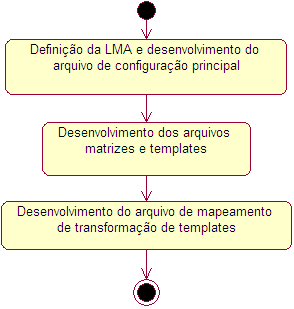
\includegraphics [width=0.45\textwidth]{res/processo}
  \caption {Processo de configura��o da ferramenta Captor}
  \label{fig:processo}
\end{figure}

Na primeira etapa da configura��o da ferramenta deve ser definido a linguagem de modelagem de aplica��es (LMA) e baseado nessa linguagem, deve ser desenvolvido o arquivo de configura��o principal contendo as defini��es dos formul�rios e das regras de valida��o da especifica��o. Na segunda etapa s�o desenvolvidos os arquivos matrizes e os templates. Na terceira etapa, o arquivo de mapeamento de transforma��o de templates � desenvolvido para indicar para a ferramenta quais templates devem ser utilizados no processo de gera��o de artefatos.

%------------------------------------------------------------------------------
%------------------------------------------------------------------------------

\subsection{Cria��o da linguagem de modelagem de aplica��es e desenvolvimento do arquivo de configura��o principal} \label{subsec:aml}

Para gerar uma aplica��o em um dom�nio particular, � necess�rio que seja modelado uma linguagem de especifica��o de aplica��es\footnote{Como entrada para o processo de modelagem da linguagem de  aplica��es, s�o necess�rios os artefatos da an�lise de dom�nio e projeto modular \cite{weiss}. A persist�ncia de dados em banco de dados relacionais � uma atividade recorrente durante a programa��o de aplica��es, e por esse motivo, este manual pretende utilizar o conhecimento do leitor no dom�nio escolhido e omitir as atividades de an�lise de dom�nio e projeto modular.}. Essa linguagem � utilizada para descrever aplica��es nesse dom�nio e a sua estrutura deve expressar os par�metros de varia��o que as aplica��es nesse dom�nio podem apresentar.

No dom�nio de persit�ncia, uma classe representa uma tabela do banco de dados e os atributos dessa classe representam uma tupla dessa tabela. As classes persistentes devem fornecer um m�todo para inserir uma tupla em uma tabela, um m�todo para recuperar uma tupla de uma tabela e um m�todo para remover uma tupla de uma tabela.

Os par�metros de varia��o necess�rios para especificar classes persistentes s�o apresentados na Tabela \ref{tab:variacao}.

\begin{table}[ht]
	\centering
	\caption{Par�metros de varia��o}
	\label{tab:variacao}
		
		\begin{tabular}{|p{105pt}|p{300pt}|}

			\hline 
			\hline 

			\hline 
			\textbf{Par�metro} &  \textbf{Descri��o} \\


			\hline 
			Nome do pacote &  O nome do pacote em que as classes devem ser armazenadas. \\
			
			\hline 
			Nome da classe &  O nome da classe persistente que deve ser criada. \\

			\hline 
			Nome da tabela &  O nome da tabela do banco de dados que essa classe representa. \\

			\hline 
			Atributos da classe & O nome dos atributos da classe persistente. \\
			 
			\hline 
			Atributos da tabela & O nome dos atributos da tabela do banco de dados. \\
			
			\hline 
			Tipos dos atributos & O tipo dos atributos da classe e da tabela. \\

			\hline 
		\end{tabular}

	\end{table}

Para simplificar este exerc�cio, uma classe n�o pode ter associa��es com outras classes e os tipos v�lidos dos atributos das classes e das tabelas s�o apenas os tipos inteiros e \textit{strings}. Como exerc�cio complementar, o leitor pode realizar a configura��o completa da ferramenta para o dom�nio de persist�ncia incluindo diversos tipos de relacionamentos entre classes e apoio para os principais tipos de dados dispon�veis nos banco de dados comerciais.

Note que a especifica��o desses par�metros de varia��o dispon�veis na Tabela \ref{tab:variacao} n�o s�o baseadas na linguagem de programa��o Java ou na interface de programa��o JDBC. O objetivo da cria��o e utiliza��o dessa linguagem � permitir que o engenheiro de aplica��o especifique uma aplica��o de forma abstrata e obtenha a diminui��o do esfor�o e tempo de desenvolvimento de aplica��es nesse dom�nio por meio da gera��o dos artefatos.

%------------------------------------------------------------------------------

Para iniciar a parte t�cnica do processo de configura��o, � necess�rio a cria��o do arquivo de configura��o principal. O arquivo de configura��o principal descreve a estrutura dos formul�rios da especifica��o, os componentes gr�ficos que cada formul�rio cont�m e as regras de valida��o dessa especifica��o. Na Figura \ref{fig:processoConfig} s�o apresentadas as principais etapasdo processo de desenvolvimento do arquivo de configura��o principal.

\begin{figure} [!ht]
 \centering
  \bfseries
  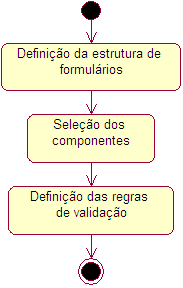
\includegraphics [width=0.30\textwidth]{res/processoConfig}
  \caption {Processo de desenvolvimento da LMA}
  \label{fig:processoConfig}
\end{figure}

%------------------------------------------------------------------------------

\subsubsection{Defini��o da estrutura de formul�rios}\label{subsec:arp}

Os formul�rios s�o estruturados na ferramenta em forma de �rvore. A especifica��o da aplica��o come�a com a edi��o de um formul�rio ra�z que pode conter um ou mais formul�rios filhos.

Baseado no conhecimento de dom�nio e no conhecimento funcional da ferramenta, pode ser definida  a seguinte estrutura de formul�rios para armazenar os par�metros de varia��o contidos na Tabela \ref{tab:variacao}:\\

Para o n� ra�z da especifica��o, pode ser definido um formul�rio com uma caixa de texto contendo a descri��o das classes de persit�ncia que est�o sendo geradas. As classes persistentes s�o agrupadas em pacotes. Os pacotes s�o especificados no n�s filhos do formul�rio ra�z. As classes persistentes s�o especificadas nos formul�rios filhos do formul�rio da especifica��o de pacotes. Os formul�rios que representam as classes persistentes devem conter um campo para especificar o nome da classe, um campo para especificar o nome da tabela que essa classe representa e um componente gr�fico em forma de tabela para descrever o nome e tipo dos atributos das classes e da tabela.

Um formul�rio de descri��o de classes pode ter um ou mais n�s filhos com descri��o de pacotes e os formul�rios de especifica��o de pacotes podem conter um ou mais n�s filhos com os formul�rios da especifica��o de classes.

Na Figura \ref{fig:formstructure} � apresentado essa estrutura de formul�rios e as Figuras \ref{fig:projectform}, \ref{fig:packageform} e \ref{fig:classform} apresentam esquematicamente os componentes gr�ficos de cada formul�rio da Figura \ref{fig:formstructure}.

\begin{figure} [!ht]
 \centering
  \bfseries
  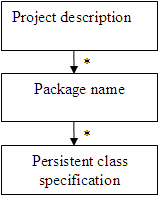
\includegraphics [width=0.30\textwidth]{res/formstructure}
  \caption {Estrutura de formul�rios}
  \label{fig:formstructure}
\end{figure}

\begin{figure} [!ht]
 \centering
  \bfseries
  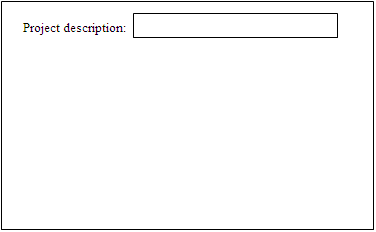
\includegraphics [width=0.55\textwidth]{res/projectform}
  \caption {Formul�rio de especifica��o da descri��o do projeto}
  \label{fig:projectform}
\end{figure}

\begin{figure} [!ht]
 \centering
  \bfseries
  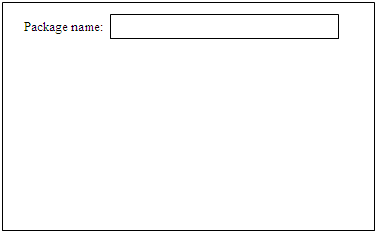
\includegraphics [width=0.55\textwidth]{res/packageform}
  \caption {Formul�rio de especifica��o de pacotes}
  \label{fig:packageform}
\end{figure}

\begin{figure} [!ht]
 \centering
  \bfseries
  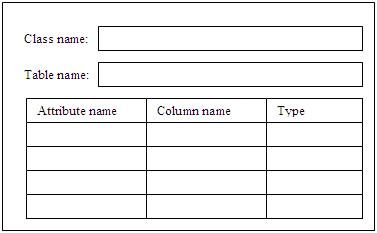
\includegraphics [width=0.55\textwidth]{res/classform}
  \caption {Formul�rio de especifica��o de classes persistentes}
  \label{fig:classform}
\end{figure}

%------------------------------------------------------------------------------

\subsubsection{Sele��o dos componentes}

Para montar os formul�rios definidos na Sub-se��o \ref{subsec:arp} � necess�rio escolher os componentes de formul�rio que cada formul�rio deve conter. Baseado nas Figuras \ref{fig:projectform}, \ref{fig:packageform} e \ref{fig:classform} e no manual de componentes de formul�rio, o engenheiro de dom�nio pode escolher os seguintes componentes:\\

\noindent\textbf{Formul�rio de descri��o de projetos}

\begin{itemize}
	\item O componente de formul�rio TextAreaPanel para definir a descri��o do projeto.
\end{itemize}

\noindent\textbf{Formul�rio de especifica��o de pacotes:}

\begin{itemize}
	\item O componente de formul�rio TextPanel para definir o nome dos pacotes.
\end{itemize}

\noindent\textbf{Formul�rio de especifica��o de classes:}

\begin{itemize}
	\item O componente de formul�rio TextPanel para definir o nome da classe.
	\item O componente de formul�rio TextPanel para definir o nome da tabela.
	\item O componente de formul�rio TablePanel para definir o nome dos atributos da classe e das tabelas, e os tipos desses atributos.
\end{itemize}

%------------------------------------------------------------------------------

\subsubsection{Defini��o das regras de valida��o}

O engenheiro de dom�nio deve configurar a ferramenta para fazer a valida��o da especifica��o da aplica��o. A defini��o das regras de valida��o tem o objetivo de n�o permitir que o engenheiro de aplica��o gere artefatos � partir de uma especifica��o inv�lida.

A ferramenta Captor fornece duas formas de valida��o: a valida��o estrutural e a valida��o sint�tica. 

A valida��o estrutural deve asssegurar que n�o exista nenhum formul�rio de especifica��o de pacotes que n�o contenha pelo menos um formul�rio filho com a especifica��o de uma classe e a valida��o sint�tica deve ser aplicada nos formul�rios de especifica��o de pacotes e nos formul�rios de especifica��o de classes. As regras de valida��o sint�tica dos dados inseridos nos componentes de formul�rio s�o apresentados na Tabela \ref{tab:validate}.

\begin{table}[ht]
	\centering
	\caption{Regras de valida��o}
	\label{tab:validate}
		
		\begin{tabular}{|p{95pt}|p{340pt}|}

			\hline 
			\hline 

			\hline 
			\textbf{Par�metro} &  \textbf{Descri��o} \\

			\hline 
			Nome do pacote &  O nome do pacote deve ser especificado de acordo com a express�o regular:\\ &([a-zA-Z]+[a-zA-Z$\backslash$-0-9]+)+([$\backslash$$\backslash$/][a-zA-Z]+[a-zA-Z$\backslash$-0-9]+)* \\

			\hline 
			Nome da classe &  O nome da classe deve ser especificada de acordo com a express�o regular:\\ & [A-Z]+([a-zA-Z$\backslash$-0-9]+)*[A-Za-z]+ \\

			\hline 
			Nome da tabela &  O nome da tabela deve ser especificada de acordo com a express�o regular:\\ & [A-Za-z]+([a-zA-Z$\backslash$-\_0-9]+)*[A-Za-z]+  \\
			
			\hline 
			Atributos da classe & O nome dos atributos da classe devem ser especificados de acordo com a express�o regular:\\ & [a-z]+([a-zA-Z$\backslash$-\_0-9]+)*[A-Za-z]+  \\
			
			\hline 
			Colunas da tabela & O nome das colunas da tabela devem ser especificados de acordo com a express�o regular:\\ & [A-Z]+([a-zA-Z$\backslash$-\_0-9]+)*[A-Za-z]+ \\
			
			\hline 
			Tipos dos atributos & Os tipos de dados devem ser especificados de acordo com a express�o regular: \\ & [int]*[String]* \\

			\hline 
		\end{tabular}

	\end{table}

%------------------------------------------------------------------------------
%------------------------------------------------------------------------------

\subsection{Desenvolvimento dos arquivos matrizes e templates}\label{subsec:templates}

Para iniciar o desenvolvimento de \textit{templates} � necess�rio que exista pelo menos um exemplo de c�digo desenvolvido manualmente. � partir desse exemplo, chamado de exemplo matriz, os \textit{templates} s�o desenvolvidos.

%------------------------------------------------------------------------------

\subsubsection{Matriz SQL}

Na Listagem \ref{lst:sql} � apresentado o c�digo SQL necess�rio para realizar a cria��o de uma tabela no banco de dados MySQL \cite{mysql}.

\lstset{language=sql}
\begin{lstlisting}[caption=C�digo SQL necess�rio para criar uma tabela do banco de dados,label=lst:sql]
CREATE TABLE NOME_DA_TABELA 
  (att1 int, att2 int, att3 varchar(50));
\end{lstlisting}

%------------------------------------------------------------------------------

\subsubsection{Matriz de classe persistente (Java - JDBC)}

A Matriz dos c�digo Java que realiza a persist�ncia de uma classe Java � apresentada na Listagem \ref{lst:java}.

\lstset{language=java}
\begin{lstlisting}[caption=C�digo Java de uma classe persistente,label=lst:java]
package exemplo.persistente;

import java.sql.*;

public class Pessoa  {

  private int id;
  private String nome;
  private int idade;
  private boolean sexo;
	
  private Connection con;
	
  public Pessoa(Connection con)  {
    nome = new String();
    idade = 0;
    id = 0;
    sexo = true;	
    this.con = con;
  }	
	
  //getters and setters
  public int getId()  {
    return id;
  }
  public void setId(int id)  {
    this.id = id;	
  }

  public String getNome()  {
    return nome;
  }
  public void setNome(String nome)  {
    this.nome = nome;	
  }
	
  public int getIdade()  {
    return idade;
  }
  public void setIdade(int idade)  {
    this.idade = idade;	
  }
	
  public boolean getSexo()  {
    return sexo;
  }
  public void setSexo(boolean sexo)  {
    this.sexo = sexo;	
  }

  //persistent methods
  public boolean save()  {
    Statement stmt = null;
		
    //create a query
    String query = ``INSERT INTO PESSOA (ID, NOME, IDADE,SEXO)'';
    query = query + ``VALUES (ID_, 'NOME_', IDADE_,'SEXO_')'';

    //create string data from class attributes
    String idString = new Integer(id).toString();
    String idadeString = new Integer(idade).toString();
    String sexoString = new Boolean(sexo).toString();
    sexoString = sexoString.substring(0,1);
    
    //put the attribute values into the query
    query = query.replaceFirst(``ID_'', idString);
    query = query.replaceFirst(``NOME_'', nome);
    query = query.replaceFirst(``IDADE_'', idadeString);
    query = query.replaceFirst(``SEXO_'', sexoString);
		
    try {
      //create and execute the statement
      stmt = con.createStatement();
      stmt.executeUpdate(query);
    			
      try {
        //close connection
        stmt.close();
        return true;
      } catch (SQLException ex) { 
        System.out.println(ex);
        return false;
      }
    }catch(Exception ex)  {
      System.out.println(ex);
      return false;
    }
  }	
  
  public boolean getById(int id)  {
    Statement stmt = null;
    ResultSet rs = null;
		
    String idString = new Integer(id).toString();

    String query = ``SELECT * FROM PESSOA WHERE ID = ID_'';
    query = query.replaceFirst(``ID_'', idString);
		
    try {
      stmt = con.createStatement();
      rs = stmt.executeQuery(query);
			
      while (rs.next() )  {
        this.id = rs.getInt(``ID'');
        nome = rs.getString(``NOME'');
        idade = rs.getInt(``IDADE'');
        String sx = rs.getString(``SEXO'');
        if ( sx.equals(``t'') )
          sexo = true;
        else
          sexo = false;
      }			
			
      try {
        stmt.close();
        return true;
      } catch (SQLException ex) { 
        System.out.println(ex);
        return false;
      }
    }catch(Exception ex)  {
      System.out.println(ex);
      return false;
    }
		
  }
	
  public boolean delete()  {
    Statement stmt = null;
		
    String idString = new Integer(id).toString();

    String query = ``DELETE FROM PESSOA WHERE ID = ID_'';
    query = query.replaceFirst(``ID_'', idString);
		
    try {
      stmt = con.createStatement();
      stmt.executeUpdate(query);
			
      try {
        stmt.close();
        return true;
      } catch (SQLException ex) { 
        System.out.println(ex);
        return false;
      }
    }catch(Exception ex)  {
      System.out.println(ex);
      return false;
    }
			
 }
	
}
\end{lstlisting}

� partir das matrizes apresentadas nas Listagens \ref{lst:sql} e \ref{lst:java}, o engenheiro de dom�nio pode iniciar o desenvolvimento dos \textit{templates}.

A linguagen de transforma��es XSL est� fora do escopo desse manual. Instru��es
detalhadas da linguagem XSL podem ser encontradas no site: http://
www.w3c.org/xslt e em diversos manuais e livros dispon�veis livremente ou para compra
na internet.

No diret�rio install\_dir/doc/training/XSLT\_examples podem ser encontrados exemplos de transforma��es XML em ordem progressiva de complexidade. Esses exemplos podem ser executados na linha de comando ou com a ferramenta Ant.

%------------------------------------------------------------------------------

\subsection{Desenvolvimento do arquivo de mapeamento de transforma��o de templates}\label{subsec:mtl}

O arquivo de mapeamento de transfoma��o de templates deve informar a ferramenta sobre a necessidade da gera��o de dois tipos de arquivos: o arquivo com os scripts SQL para a cria��o das tabelas no banco de dados e as classes Java persistentes.

Para cada projeto deve ser gerado um script SQL e dentro de um projeto, para cada especifica��o de classe persistente, deve ser criado um arquivo com o nome igual ao nome da classe definida no formul�rio de especifica��o de classes.

%------------------------------------------------------------------------------

\subsection{Exerc�cio 1: Configura��o da ferramenta}\label{subsec:exercicio1}

Na primeira parte do exerc�cio, o leitor deve configurar a ferramenta Captor com base nos dados fornecidos nesta Se��o. As atividades neecess�rias para completar o exerc�cio s�o:

\begin{enumerate}
	\item Criar o arquivo de configura��o principal com a defini��o dos formul�rios e dos mecanismos de valida��o.
	\item Criar os templates para gerar o c�digo SQL e os templates para o C�digo Java.
	\item Criar o arquivo de mapeamento de transforma��o de templates.
	\item Implantar os artefatos criados na ferramenta.
	\item Testar a nova configura��o.
\end{enumerate}

%------------------------------------------------------------------------------

\section{Utiliza��o da ferramenta}\label{sec:utilizar}

Para utilizar a ferramenta, o engenheiro de aplica��o deve possuir a especifica��o de requisitos de uma aplica��o em um dom�nio que a ferramenta forne�a apoio, editar os dados dessa especifica��o na ferramenta, gerar artefatos e utilizar esses artefatos no desenvolvimento de aplica��es.

\subsection{Exerc�cio 2 - Utiliza��o da ferramenta}\label{subsec:exercicio2}

O estudo conduzido nesse exerc�cio deve implementar as classes persistentes para as tabelas relacionais apresentadas na Figura \ref{fig:tabelasrelacionais}.

\begin{figure} [!ht]
 \centering
  \bfseries
  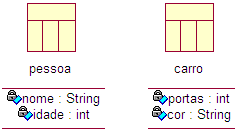
\includegraphics [width=0.45\textwidth]{res/tabelasrelacionais}
  \caption {Tabelas relacionais da aplica��o exemplo}
  \label{fig:tabelasrelacionais}
\end{figure}

As tabelas relacionais apresentadas na Figura \ref{fig:tabelasrelacionais} s�o mapeadas para as classes persistentes apresentadas na Figura \ref{fig:uml}.

\begin{figure} [!ht]
 \centering
  \bfseries
  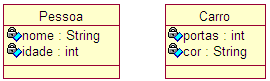
\includegraphics [width=0.45\textwidth]{res/uml}
  \caption {Classes persitentes}
  \label{fig:uml}
\end{figure}

Para o exerc�cio de utiliza��o da ferramenta Captor s�o propostas as seguintes atividades:

\begin{itemize}
	\item Edi��o de uma especifica��o da ferramenta Captor que represente as tabelas e classes apresentadas nas Figuras \ref{fig:tabelasrelacionais} e \ref{fig:uml}.
	\item Gera��o dos artefatos.
	\item Teste dos artefatos gerados.
	\item Cria��o de zonas de seguran�a nos templates para adi��o de novos m�todos nas classes geradas.
	\item Modifica��o dos artefatos gerados dentro das zonas de seguran�a.
\end{itemize}

%------------------------------------------------------------------------------


%******************  Bibliografia  ********************************************

\newpage
\renewcommand{\bibname}{Refer�ncias}
\bibliography{res/refs}

\addcontentsline{toc}{section}{\bibname}

%***************************************

\end{document}

